\documentclass[10pt,letterpaper]{book}

\usepackage[top=1.25in, bottom=1.25in, left=1.33in, right=1.33in]{geometry}
\usepackage{amsmath}
\usepackage[all]{xy}
\usepackage{graphicx}

\newcommand{\ulex}{\texttt{ml-ulex}}
\newcommand{\mlantlr}{\texttt{ml-antlr}}
\newcommand{\antlr}{\texttt{ml-antlr}}

\title{SML/NJ Language Processing Tools\\
DRAFT}
\author{Aaron Turon\\
\texttt{adrassi@cs.uchicago.edu}}
%\date{ }

\newcommand{\Carat}{\^{ }}
\newcommand{\RE}{r}
\newcommand{\OR}{\ | \ }
\newcommand{\AND}{\ \& \ }
\newcommand{\CL}{\mathcal{L}}
\newcommand{\CS}{\mathcal{S}}
\newcommand{\CR}{\mathcal{R}}
\newcommand{\CP}{\mathcal{P}}
\newcommand{\Sem}[1]{[ \! [ #1 ] \! ]}
\newcommand{\Ls}[1]{\CL\Sem{#1}}

\newcommand{\eg}{{\em e.g.}}
\newcommand{\cf}{{\em cf.}}
\newcommand{\ie}{{\em i.e.}}

\newcommand{\nm}[1]{\texttt{#1}}

\newcommand{\ra}{\rightarrow}
\newcommand{\Ra}{\Rightarrow}

\newcommand{\New}[1]{\emph{\textbf{#1}}}

% Grammar
\newcommand{\Grammar}[1]{\[ \begin{array}{rcll} #1 \end{array} \]}
\newcommand{\GFirst}[3]{#1 & ::= & #2 & \textrm{#3} \\ }
\newcommand{\GNext}[2]{ & | & #1 & \textrm{#2} \\ }

\newcommand{\GFirstB}[2]{\textit{#1} & ::= & \multicolumn{2}{l}{\textit{#2}} \\ }
\newcommand{\GNextB}[1]{ & | & \multicolumn{2}{l}{\textit{#1}} \\ }

\newcommand{\GFirstC}[3]{\textit{#1} & ::= & \textit{#2} & \textrm{#3} \\ }
\newcommand{\GNextC}[2]{ & | & \textit{#1} & \textrm{#2} \\ }

%\newcommand{\T}[1]{{\tt '#1'}}
\newcommand{\T}[1]{{\textbf{\tt #1}}}
\newcommand{\kw}[1]{{\T{\%#1}}}

\usepackage{amsthm}

\newtheorem*{theorem}{Theorem}
\newtheorem*{definition}{Definition}
\newtheorem*{remark}{Remark}

\usepackage{ifpdf}

\usepackage{mathpazo}
\renewcommand{\ttdefault}{cmtt}

\newcommand{\parttext}{}
\newcommand{\cpart}[1]{\renewcommand{\parttext}{#1}\part{#1}}

\usepackage{fancyhdr}

\begin{document}

\frontmatter

	\maketitle
	
	\phantom{.}
	\vspace{\stretch{1}}
	
	\noindent Copyright \copyright{}2006.  All rights reserved.
	
	\vskip 12pt
	\noindent This document was written with support from NSF grant CNS-0454136, ``CRI: Standard ML Software Infrastructure.''
	
	\pagebreak
	
	\tableofcontents

\mainmatter

	\renewcommand{\chaptermark}[1]{\markboth{#1}{}}
	\renewcommand{\sectionmark}[1]{\markright{\thesection. \ #1}{}}

    \newpage
    \phantom{.}
	\vskip 72pt
	\begin{center}
	{\Huge Notice}
	\end{center}
	\vskip 20pt \noindent
	{\Large This is an \textbf{early draft} manual for {\tt ml-ulex} and {\tt ml-antlr}.  The early release of these tools and this manual is intended for gathering feedback.  The interfaces described herein will likely undergo substantial revision before the 1.0 release of these tools.}
	
	\newpage

	\chapter{Overview}\label{chap:overview}

In software, language recognition is ubiquitous: nearly every program deals at some level with structured input given in textual form.  The simplest recognition problems can be solved directly, but as the complexity of the language grows, recognition and processing become more difficult.  

Although sophisticated language processing is sometimes done by hand, the use of scanner and parser generators\footnote{
  ``Scanner generator'' and ``parser generator'' will often be shortened to ``scanner'' and ``parser'' respectively.  This is justified by viewing a parser generator as a parameterized parser.
} is more common.  The Unix tools {\tt lex} and {\tt yacc} are the archetypical examples of such generators.  Tradition has it that when a new programming language is introduced, new scanner and parser generators are written in that language, and generate code for that language.  Traditional \emph{also} has it that the new tools are modeled after the old {\tt lex} and {\tt yacc} tools, both in terms of the algorithms used, and often the syntax as well.  The language Standard ML is no exception: {\tt ml-lex} and {\tt ml-yacc} are the SML incarnations of the old Unix tools.

This manual describes two new tools, \ulex{} and \mlantlr{}, that follow tradition in separating scanning from parsing, but break from tradition in their implementation: \ulex{} is based on \emph{regular expression derivatives} rather than subset-construction, and \mlantlr{} is based on $LL(k)$ parsing rather than $LALR(1)$ parsing.   

\section{Motivation}

Most parser generators use some variation on $LR$ parsing, a form of \emph{bottom-up} parsing that tracks possible interpretations (reductions) of an input phrase until only a single reduction is possible.  While this is a powerful technique, it has the following downsides:
\begin{itemize}
  \item Compared to predictive parsing, it is more complicated and difficult to understand.  This is particularly troublesome when debugging an $LR$-ambiguous grammar.
  \item Because reductions take place as late as possible, the choice of reduction cannot depend on any semantic information; such information would only become available \emph{after} the choice was made.
  \item Similarly, information flow in the parser is strictly bottom-up.  For (syntactic or semantic) context to influence a semantic action, higher-order programming is necessary.
\end{itemize} 
The main alternative to $LR$ parsing is the top-down, $LL$ approach, which is commonly used for hand-coded parsers.  An $LL$ parser, when faced with a decision point in the grammar, utilizes lookahead to unambiguously predict the correct interpretation of the input.  As a result, $LL$ parsers do not suffer from the problems above.  $LL$ parsers have been considered impractical because the size of their prediction table is exponential in $k$ --- the number of tokens to look ahead --- and many languages need $k > 1$.  However, Parr showed that an approximate form of lookahead, using tables linear in $k$, is usually sufficient.

To date, the only mature $LL$ parser based on Parr's technique is his own parser, {\tt antlr}.  While {\tt antlr} is sophisticated and robust, it is designed for and best used within imperative languages.  The primary motivation for the tools this manual describes is to bring practical $LL$ parsing to a functional language.
Our hope with \ulex{} and \mlantlr{} is to modernize and improve the Standard ML language processing infrastructure, while demonstrating the effectiveness of regular expression derivatives and $LL(k)$ parsing.  The tools are more powerful than their predecessors, and they raise the level of discourse in language processing.  

%\section{Outline}

%This manual is organized into three parts: usage, theory, and implementation.  Each of these parts is further broken down into two chapters, one on \ulex{} and one on \mlantlr{}.  The usage section is self-contained, and gives a fairly complete specification of the two tools.  Full details on the algorithms used are given in the theory section.  Data structures, system organization, and other code-related particulars are described in the implementation section.
	
	\renewcommand{\chaptermark}[1]{\markboth{\parttext{}: #1}{}}

	\cpart{Usage}
	
		\chapter[\ulex]{Usage: \ulex}

\section{Overview}

\textsc{ml-ulex} is used for generating ``lexers,'' which analyze the lexical structure of an input string, in this case using regular expressions..  If the generated module is called {\tt Lexer}, it will contain a type {\tt strm} and a function
\begin{verbatim}
    val lex : strm -> (token * strm) option
\end{verbatim}
where {\tt token} is a type determined by the user of \ulex{}.  Thus, a lexer is a token reader, in the sense of the Basis library {\tt StringCvt.reader} type.

The tool is invoked from the command-line as follows:
\begin{verbatim}
    ml-ulex [options] file
\end{verbatim}
where {\tt file} is the name of the input \ulex{} specification, and where {\tt options} may be any combination of:

\vskip 12pt
\begin{tabular}{lp{0.65\textwidth}}
  {\tt --dot} & generate DOT output (for graphviz; see \texttt{http://www.graphviz.org}).  The produced file will be named {\tt file.dot}, where {\tt file} is the input file. \\
  \\
  {\tt --match} & enter interactive matching mode.  This will allow interactive testing of the machine; presently, only the {\tt INITIAL} start state is available for testing (see Section~\ref{sec:start-states} for details on start states).  \\
  \\
  {\tt --ml-lex-mode} & operate in {\tt ml-lex} compatibility mode.  See Section~\ref{sec:lex-compat} for details.
%  {\tt --minimize} & generate a minimal machine.  Note that this is slow, and is almost never necessary.
\end{tabular}

\section{Specification format}

A \ulex{} specification is a list of semicolon-terminated \emph{declarations}.  Each declaration is either a \emph{directive} or a \emph{rule}.  Directives are used to alter global specification properties (such as the name of the module that will be generated) or to define named regular expressions.  Rules specify the actual reguluar expressions to be matched.  The top-level grammar is given in Figure~\ref{fig:ulex-syntax}.

\begin{figure}
\Grammar{
\GFirstB{spec}
	{$($ declaration \T{;} $)^*$}

\GFirstB{declaration}
	{directive}
\GNextB
	{rule}

%\GFirstB{directive}
%	{\kw{charset} $($ \T{ASCII7} $|$ \T{ASCII8} $|$ \T{UTF8} $)$}

\GNextB
	{\kw{defs} code}
\GNextB
	{\kw{let} ID \T{=} re}
\GNextB
	{\kw{name} ID}
\GNextB
	{\kw{states} ID$^+$}
	
\GFirstB{code}
	{ \T{(} $\dots$ \T{)} }
	
\GFirstB{rule}
	{ $($\T{<} ID $($ \T{,} ID $)^*$ \T{>}$)^?$ re \T{=>} code}
}
\caption{The top-level \ulex{} grammar}\label{fig:ulex-syntax}
\end{figure}

There are a few lexical details of the specification format worth mentioning.  First, SML-style comments (\texttt{(* ... *)}) are treated as ignored whitespace anywhere they occur in the specification, \emph{except} in segments of code.  The \textit{ID} symbol used in the grammar stands for alpha-numeric-underscore identifiers, starting with an alpha character.  The \textit{code} production represents a segment of SML code, enclosed in parentheses.  Extra parentheses occuring within strings or comments in code need not be balanced.

\section{Directives}

\subsection{The \kw{defs} directive}

The \kw{defs} directive is used to include a segment of code in the generated lexer module.  All definitions given will be in scope for the rule actions; see Section~\ref{sec:ulex-rules}.

\subsection{The \kw{let} directive}

Use \kw{let} to define named abbreviations for regular expressions; once bound, an abbreviation can be used in further \kw{let}-bindings or in rules.  For example,
\begin{verbatim}
    %let digit = [0-9];
\end{verbatim}
introduces an abbreviation for a regular expression matching a single digit.  To use abbreviations, enclose their name in curly braces.  For example, an additional \kw{let} definition can be given in terms of \texttt{digit},
\begin{verbatim}
    %let int = {digit}+;
\end{verbatim}
which matches arbitrary-length integers.  Note that scoping of let-bindings follows standard SML rules, so that the definition of \texttt{int} must appear after the definition of \texttt{digit}.

\subsection{The \kw{name} directive}

The name to use for the generated lexer module is specified using \kw{name}.

\subsection{The \kw{states} directive}

It is often helpful for a lexer to have multiple \emph{start states}, which influence the regular expressions that the lexer will match.  For instance, after seeing a double-quote, the lexer might switch into a \texttt{STRING} start state, which contains only the rules necessary for matching strings, and which returns to the standard start state after the closing quote.

Start states are introduced via \kw{states}, and are named using standard identifiers.  There is always an implicit, default start state called \texttt{INITIAL}.  Within a rule action, the function \texttt{YYBEGIN} can be applied to the name of a start state to switch the lexer into that state; see~\ref{sec:ulex-actions} for details on rule actions.

\section{Rules}\label{sec:ulex-rules}

Recall that the \texttt{lex} function of the generated lexer module is a ``token'' reader.  In general, when \texttt{lex} is applied to an input stream, it will attempt to match a prefix of the input with a regular expression given in one of the rules.  When a rule is matched, its \emph{action} (associated code) is evaluated and the result is returned.  Hence, all actions must belong to the same type, but no restrictions are placed on what that type is.

Rules are specified by an optional list of start states, a regular expression, and the action code.  The rule is said to ``belong'' to the start states it lists.  If no start states are specified, the rule belongs to \emph{all} defined start states.

Rule matching is influenced by three factors: start state, match length, and rule order.  A rule is only considered for matching if it belongs to the lexer's current start state.  If multiple rules match an input prefix, the rule matching the longest prefix is selected.  In the case of a tie, the rule appearing first in the specification is selected.

For example, suppose the start state {\tt FOO} is defined, and the following rules appear, with no other rules belonging to {\tt FOO}:
\begin{verbatim}
    <FOO> a+    => ( Tokens.as );
    <FOO> a+b+  => ( Tokens.asbs );
    <FOO> a+bb* => ( Tokens.asbs );
\end{verbatim}
If the current start state is not {\tt FOO}, none of the rules will be considered.  Otherwise, on input ``aabbbc'' all three rules are possible matches.  The first rule is discarded, since the others match a longer prefix.  The second rule is then selected, because it matches the same prefix as the third rule, but appears earlier in the specification.

\subsection{Regular expression syntax}

\begin{figure}
\Grammar{	
\GFirstB{re}
	{{\rm any nonreserved, nonwhitespace character or escape code}}
\GNextB
	{{\rm a double-quoted string, as in SML}}
\GNextC
	{\T{\{} ID \T{\}}}	{\kw{let}-bound abbreviation}
\GNextC
	{\T{[} \T{\^{ }}$^?$ $($ char \T{-} char $|$ char $)^+$ \T{]} \quad\phantom{.}}
				{a character class}
\GNextC
	{\T{.}}			{wildcard (all single charcters except texttt{{$\backslash$}n})}
\GNextB
	{\T{(} re \T{)}}
\GNextC
	{re \T{*}}		{Kleene-closure (0 or more)}
\GNextC
	{re \T{?}}		{Optional (0 or 1)}
\GNextC
	{re \T{+}}		{Positive-closure (1 or more)}
\GNextC
	{re \T{\{} INT \T{\}}}	{Match exactly {\it INT} repetitions}
\GNextC
	{re re}			{Concatenation}
\GNextC
	{\T{\^{ }} re}		{Negation (anything except \textit{re})}
\GNextC
	{re \T{\&} re}		{Intersection}
\GNextC
	{re \T{|} re}		{Union}
%\GNextB
%	{re \T{/} re}
%\GNextB
%	{re \T{\$}}
%\GNextB
%	{\T{\_}}
}
\caption{The \ulex{} grammar for regular expressions}\label{ulex-rule-syntax}
\end{figure}

The syntax of regular expressions is given in Figure~\ref{ulex-rule-syntax}; constructs are listed in precedence order, from most tightly-binding to least.  Escape codes are the same as in SML, but also include \texttt{$\backslash$uxxxx} and \texttt{$\backslash$Uxxxxxxxx}, where \texttt{xxxx} represents a hexidecimal number which in turn represents a Unicode symbol.  The specification format itself freely accepts Unicode characters, and they may be used within a quoted string, or by themselves.

Some examples:
\[
\begin{array}{rcl}
{\tt 0 | 1 | 2 | 3}	& \textit{denotes} &
    \{ \texttt{0}, \texttt{1}, \texttt{2}, \texttt{3} \}	\\
{\tt [0123]}	& \textit{denotes} &
    \{ \texttt{0}, \texttt{1}, \texttt{2}, \texttt{3} \}	\\
{\tt 0123}	& \textit{denotes} &
    \{ \texttt{0123} \}						\\
{\tt 0*}	& \textit{denotes} &
    \{ \epsilon, \texttt{0}, \texttt{00}, \dots \}		\\
{\tt 00*}	& \textit{denotes} &
    \{ \texttt{0}, \texttt{00}, \dots \}		\\
{\tt 0+}	& \textit{denotes} &
    \{ \texttt{0}, \texttt{00}, \dots \}		\\
{\tt [0-9]\{3\}}	& \textit{denotes} &
    \{ \texttt{000}, \texttt{001}, \texttt{002}, \dots, \texttt{999} \}	\\
{\tt 0* \& (..)*}	& \textit{denotes} &
    \{ \epsilon, \texttt{00}, \texttt{0000}, \dots \}	\\
\texttt{\^{ }(abc)}	& \textit{denotes} &
    \Sigma^* \setminus \{ \texttt{abc} \}
\end{array}
\]

\subsection{Actions}\label{sec:ulex-actions}

Actions are arbitrary SML code enclosed in parentheses.  The following names are in scope:
\vskip 12pt
\begin{tabular}{lp{0.65\textwidth}}
  {\tt YYBEGIN} & a function taking a start state and returning unit; changes to that start state.	\\
  {\tt yytext} & the matched text as a string.	\\
  {\tt yysubstr} & the matched text as a substring (avoids copying).	\\
  {\tt yyunicode} & the matched \emph{Unicode} text as a list of Word32.words \\
  {\tt continue} & a unit to ``token'' function which recursively calls the lexer on the input following the matched prefix, and returns its result.	\\
  {\tt yylineno} & the current line number, starting from 0.	\\
  {\tt yypos} & the current character, starting from 0.	\\
  ? & any name bound in the \kw{defs} section.
\end{tabular}

\section{Using the generated code}

The generated lexer module has a signature including the following:
\begin{verbatim}
  type prestrm
  type strm = prestrm * start_state
  val streamify : (int -> string) -> strm
  val lex : strm -> (token, strm) option
\end{verbatim}
where \texttt{token} is the result type of the lexer actions, and \texttt{start\_state} is an algebraic datatype with nullary constructors for each defined start state.  In this interface, lexer start states are conceptually part of the input stream; thus, from an external viewpoint start states can be totally ignored.  However, it is sometimes easier to control the lexer start state externally, since more contextual information may be available.  This is why the \texttt{strm} type includes a concrete \texttt{start\_state} component.

\section{An example}
\begin{verbatim}
%name CalcLex;

%let digit = [0-9];
%let int = {digit}+;
%let alpha = [a-zA-Z];
%let id = {alpha}({alpha} | {digit})*;

%defs (
  open CalcParse.Tok
);

let     => ( KW_let );
in      => ( KW_in );
{id}    => ( ID (yytext()) );
{int}   => ( NUM (valOf (Int.fromString (yytext()))) );
"="     => ( EQ );
"+"     => ( PLUS );
"-"     => ( MINUS );
"*"     => ( TIMES );
"("     => ( LP );
")"     => ( RP );
" " | \n | \t
        => ( continue() );
.       => ( (* handle error *) );
\end{verbatim}

\section{{\tt ml-lex} compatibility}\label{sec:lex-compat}

Running \ulex{} with the {\tt --ml-lex-mode} option will cause it to process its input file using the ML-Lex format, and interpret the actions in a ML-Lex-compatible way.  The compatibility extends to the bugs in ML-Lex, so in particular \texttt{yylineno} starts at 2 in {\tt --ml-lex-mode}.
		\chapter[\mlantlr]{Usage: \mlantlr}

\section{Overview}

\section{Specification format}

\Grammar{
\GFirstB{spec}
	{$($ declaration \T{;} $)^*$}

\GFirstB{declaration}
	{directive}
\GNextB
	{nonterminal}

\GFirstB{directive}
	{\kw{defs} code}
\GNextB
	{\kw{import} STRING}
\GNextB
	{\kw{keywords} symbol$^+$}
\GNextB
	{\kw{name} ID}
\GNextB
	{\kw{start} ID}
\GNextB
	{\kw{tokens} \T{:} tokdef $($ \T{|} tokdef $)^*$}
	
\GFirstB{code}
	{ \T{(} $\dots$ \T{)} }

\GFirstB{tokdef}
	{datacon $($ \T{(} STRING \T{)} $)^?$}

\GFirstB{datacon}
	{ID}
\GNextB
	{ID \T{of} monotype}
\GFirstB{monotype}
	{{\rm usual SML syntax}}

\GFirstB{symbol}
	{ID}
\GNextB
	{STRING}
}

\Grammar{
\GFirstB{nonterminal}
	{ntdef}
\GNextB
	{\kw{extend} ntdef}
\GNextB
	{\kw{replace} ntdef}
\GNextB
	{\kw{drop} ID$^+$}
	
\GFirstB{ntdef}
	{ID formals$^?$ \T{:} prodlist}

\GFirstB{formals}
	{ \T{(} ID $($ \T{,} ID $)^*$ \T{)} }
	
\GFirstB{prodlist}
	{production $($ \T{|} production $)^*$}
	
\GFirstB{production}
	{\kw{try}$^?$ named-item$^*$ $($ \T{=>} code $)^?$ $($ \kw{where} code
$)^?$}
\GFirstB{named-item}
	{$($ ID \T{:} $)^?$ item}
\GFirstB{item}
	{prim-item \T{?}}
\GNextB
	{prim-item \T{+}}
\GNextB
	{prim-item \T{*}}
	
\GFirstB{prim-item}
	{symbol args$^?$}
\GNextB
	{ \T{(} prodlist \T{)} }
	
\GFirstB{args}
	{\T{@} code}
}


\section{An example}

\begin{verbatim}
calc.grm

%name CalcParse;
%tokens
  : KW_let  ("let")  | KW_in   ("in")
  | ID of string     | NUM of Int.int
  | EQ      ("=")    | PLUS    ("+")
  | TIMES   ("*")    | MINUS   ("-")
  | LP      ("(")    | RP      (")")
  ;

exp(env)
  : "let" ID "=" exp@(env) 
    "in" exp@(AtomMap.insert(env, Atom.atom ID, exp1))
      => ( exp2 )
  | addExp@(env)
  ;

addExp(env)
  : multExp@(env) ("+" multExp@(env))*
      => ( List.foldl op+ multExp SR1 )
  ;

multExp(env)
  : prefixExp@(env) ("*" prefixExp@(env))*
      => ( List.foldl op* prefixExp SR1 )
  ;

prefixExp(env)
  : atomicExp@(env)
  | "-" prefixExp@(env)
      => ( ~prefixExp )
  ;

atomicExp(env)
  : ID  
      => ( valOf(AtomMap.find (env, Atom.atom ID)) )
  | NUM
  | "(" exp@(env) ")"
  ;
\end{verbatim}

	
	\cpart{Theory}
	
		\chapter[\ulex]{Theory: \ulex}\label{sec:theory}

{\Large NOTE: this chapter has been integrated into a paper, and thereafter much improved.  In the near future, the paper will be re-adapted to replace this chapter.}

\section{Regular expressions}

Throughout this section, we assume an \emph{alphabet} $\Sigma$; any $a \in \Sigma$ is a \emph{symbol}.  Since we support unicode, $\Sigma$ can be quite large.  Our abstract regular expression (RE) language is as follows:

\Grammar{
\GFirst{\rm RE}{\epsilon}{empty string}
\GNext{\CS}{symbol set, $\CS \subseteq \Sigma$}
\GNext{\rm RE\cdot RE}{concatenation}
\GNext{\rm RE^*}{Kleene-closure}
\GNext{\rm RE \OR RE}{alternation (union)}
\GNext{\rm RE \AND RE}{intersection}
\GNext{\neg \rm RE}{negation}
}

Note that we treat symbol sets (\ie{}, character classes) as primitive; this matches the implementation strategy and simplifies the description of DFA generation.  With this representation, the empty set $\emptyset$ and the alphabet $\Sigma$ are both treated as symbol sets.  The former will yield an RE that matches no input (\ie{}, $\CL\Sem{\emptyset} = \emptyset$), and the latter will match any single symbol.  Notice also that our language of REs allows for intersection and negation in addition to the standard operations.

The semantics of our RE language are given in the form of a function $\Ls{-} \ : \ \mathrm{RE} \rightarrow \Sigma^*$ from REs to their corresponding language over $\Sigma$:

\begin{eqnarray*}
\Ls{\epsilon} 	&=& 	\epsilon \\
\Ls{\CS}		&=& 	\CS \\
\Ls{r\cdot s}	&=& 	\Ls{r} \cdot \Ls{s} \\
\Ls{r^*}		&=& 	\epsilon \cup \Ls{r}\cdot\Ls{r^*} \\
\Ls{r \OR s}	&=&		\Ls{r} \cup \Ls{s} \\
\Ls{r \AND s}	&=& 	\Ls{r} \cap \Ls{s} \\
\Ls{\neg r}		&=& 	\Sigma \setminus \Ls{r}
\end{eqnarray*}

\section{Derivatives}\label{sec:derivatives}

Brzozowski introduced \emph{derivatives} of regular expressions as an alternative means of DFA construction \cite{derivatives}.  His approach is attrative because it easily allows the language of REs to be extended with arbitrary boolean operations.  Further, it is intuitive, relatively easy to implement, goes directly from an RE to a DFA, and with some care in implementation can be made competitive with other DFA construction approaches.  We begin by introducing the notion of a derivative of some language $\CL$.

\begin{definition}  The \New{derivative} of a set of symbol sequences $\CL \subset \Sigma^*$ with respect to a finite symbol sequence $u$ is defined to be $D_u(\CL) = \{ v \ | \ u\cdot v \in \CL \}$.
\end{definition} 

Derivatives give a very natural algorithm for DFA construction.  Before giving that algorithm, however, we need a means of computing derivatives for regular expressions.

\begin{definition} A regular expression $\RE$ is \New{nullable} if the language it defines contains the empty string, that is, if $\epsilon \in \Ls{\RE}$.
\end{definition}

We also need the following function:
\[ \delta(\RE) =
    \begin{cases}
        \epsilon & \textrm{if} \ \epsilon \in \CL\Sem{\RE} \\
        \emptyset & \textrm{if} \ \epsilon \notin \CL\Sem{\RE}
    \end{cases}
\]
The $\delta$ function takes REs to REs (recall that the empty set is a symbol set, which is an RE).  Intuitively, $\delta$ collapses an RE to the ``smallest'' RE with the same nullability.

The following function, due to Brzozowski, gives the derivative of a regular expression with respect to a symbol $a$.  
\begin{eqnarray*}
D_a (\epsilon)  &=& \emptyset \\
D_a (\CS)         &=& 
    \begin{cases}
        \epsilon & \textrm{if} \ a \in \CS \\
        \emptyset & \textrm{if} \ a \notin \CS \\
    \end{cases} \\
D_a (r \cdot s) &=& D_a(r)\cdot s \OR \delta(r) \cdot D_a(s) \\
D_a (r^*)       &=& D_a(r) \cdot r^* \\
D_a (r \OR s)   &=& D_a(r) \OR D_a(s) \\
D_a (r \AND s)  &=& D_a(r) \AND D_a(s) \\
D_a (\neg r)    &=& \neg D_a(r)
\end{eqnarray*}

We can take the derivative of an RE with respect to a sequence of symbols in a straightforward way:
\begin{eqnarray*}
D_\epsilon (r) &=& r \\
D_{ua} (r) &=& D_a(D_u(r))
\end{eqnarray*}

Intuitively, the derivative of an RE with respect to a symbol $a$ yields a new RE after matching $a$.  The following two theorems, again due to Brzozowski, make this precise.

\begin{theorem} The derivative $D_s(\RE)$ of any regular expression $\RE$ with respect to any sequence $u$ is a regular expression.
\end{theorem}

\begin{theorem} A sequence $u$ is contained in $\Ls{\RE}$ if and only if $\Ls{D_u(\RE)}$ is nullable.
\end{theorem}

Derivatives provide an easy method of DFA construction.  Suppose we want to build a DFA that recognizes $\RE$.  We can think of each state of the DFA as a regular expression.  We start with a state $Q_0$ that represents $\RE$.  We then take the derivative of $\RE$ with respect to each symbol of the alphabet and create a new state each time a new derivative is found, adding each new state to the work list.  We pop a state from the work list and repeat, until the work list is empty.  There will be a transition from $Q_j$ to $Q_k$ if and only if (identifying states and their REs) $D_a (Q_j) = Q_k$ for some symbol $a$; the transition will be labeled with the set of all such $a$.  Finally, any state that represents a nullable RE is an accepting state.  The correctness of the recognizer is a direct consequence of the above theorems.

The sketch glosses over several important details.  First, what notion of equality do we intend for the equation $D_a (Q_j) = Q_k$?  Ideally, we would identify as a single state all those REs which admit the same language, so that $D_a (Q_j) = Q_k$ if and only if $\Ls{D_a (Q_j)} = \Ls{Q_k}$.  This is expensive to compute, so Brzozowski introduced the notion of RE similarity, an equivalence on REs which is easy to compute but still guarantees that the DFA is finite.

Let $\approx$ denote the least equivalence relation on REs such that
\begin{eqnarray*}
r \OR r &\approx& r \\
r \OR s &\approx& s \OR r \\
(r \OR s) \OR t &\approx& r \OR (s \OR t)
\end{eqnarray*}

\begin{definition} Two regular expressions $r$ and $s$ are \New{similar} if $r \approx s$ and are \New{dissimilar} otherwise.
\end{definition}

\begin{theorem} Every regular expression has only a finite number of dissimilar derivatives.
\end{theorem}

Hence, DFA construction is guaranteed to succeed if new states are only created when no existing state is similar to a given derivative.  In fact, we want to do much better then this to avoid blowup in DFA size.

\begin{remark}
In a practical implementation of DFA construction using derivatives, it is crucial to aggresively identify when a derivative admits the same language as an existing state (RE) in the DFA.  The cost of this identification must be balanced against the number of duplicate states avoided.
\end{remark}

In \ulex{}, we accomplish this by canonicalizing all input and derived REs.  The canonicalization is described in detail in section~\ref{sec:reg-exp}.

\section{Factorings}\label{sec:factorings}

Another problem with DFA construction is the size of the unicode alphabet: taking the derivative with respect to each unicode symbol is not feasible.  But to construct the DFA, we have to examine every possible derivative of a given RE.  We must try to conservatively estimate what sets of symbols will yield the same derivative for an RE.  Here we break from Brzozowski's work and introduce new terminology and an algorithm to make derivatives more amenable to large alphabets.

Let $\sim_\RE$ be the relation defined as follows.  For a regular expression $\RE$ and symbols $a, b$, $a \sim_\RE b$ if and only if $D_a (\RE) = D_b (\RE)$.

\begin{definition}
The \New{derivative classes} of $\RE$ are the the equivalence classes $\Sigma/{\sim_\RE}$.
\end{definition}

Ultimately, the outedges for a DFA state and the derivative classes of the RE for that state are in one-to-one correspondence.\footnote{This is not quite true: we usually drop error transitions, that is, transitions going to the RE $\emptyset$.}   Hence, we must eventually determine all the derivative classes for an RE in order to construct the DFA.  To avoid testing the entire alphabet a symbol at a time, we introduce an algorithm which (over)partitions $\Sigma$, so that each partition is a subset of a derivative class.   We can then take the derivative with respect to a representative from each partition, and determine which partitions actually belong to the same derivative class.

\begin{definition}
Let $r$ be an RE.  A \New{factoring} of $\Sigma$ under $r$ is a partitioning of $\Sigma$ such that each partition is a subset of a derivative class for $\RE$.
\end{definition}

To be clear: we are factoring the \emph{alphabet} into partitions, but the factoring is guided by (\emph{under}) a regular expression.  A factoring under a given RE is not unique.  The derivative classes for an RE are one possible factoring (with a minimal number of partitions) while the set of all singleton sets of symbols is another factoring (with a maximal number of partitions).  We will present a simple recursive factoring algorithm and prove its correctness, but first, an example.

Suppose we have two regular expressions $r$ and $s$ yielding factorings $\{ \CR_1, \CR_2 \}$ and $\{ \CS_1, \CS_2 \}$ respectively.  Let $t = r \OR s$.  The derivative of $t$ with respect to some symbol $a$ is $D_a(t) = D_a(r) \OR D_a(s)$.  Hence, if $D_a(r) = D_b(r)$ and $D_a(s) = D_b(s)$ for some symbols $a, b$, then $D_a(t) = D_b(t)$ and so $a \sim_t b$.  We can use this to give a factoring under $t$.  The relationship between the factorings under $r$, $s$ and $t$ can be visualized as follows:

\[
  \xymatrix{
    \bullet \ar@{-}[rrr]|{\Sigma} &&& \bullet \\
    \bullet \ar@{-}[rr]|{\CR_1} && \bullet \ar@{-}[r]|{\CR_2} & \bullet \\
    \bullet \ar@{-}[r]|{\CS_1} & \bullet \ar@{-}[rr]|{\CS_2} &&  \bullet \\
    \bullet \ar@{-}[r]|{\CR_1 \cap \CS_1} & 
    \bullet \ar@{-}[r]|{\CR_1 \cap \CS_2} & 
    \bullet \ar@{-}[r]|{\CR_2 \cap \CS_2} &
    \bullet
  }
\]

This small example captures the essential idea of the algorithm.  To give a factoring under an RE, we recursively find factorings under its components and ``compress'' those factorings into a single new factoring that respects them.  The factorings are being compressed (flattened) in the sense that the boundaries of one factoring are forced onto another, causing some partitions to split.  The algorithm we present is in two stages: first, a factoring function recurively collects factorings under an RE; then, a compress function compresses them all onto $\Sigma$ to produce a single factoring for an RE.  We now make this precise.

The \emph{factoring} function $F$ takes a regular expression and gives a factoring of $\Sigma$ under that RE.  It is defined recursively as follows:
\begin{eqnarray*}
F(\epsilon)     &=& \emptyset \\
F(\CS)          &=& \{ \CS \} \\
F(r \cdot s)    &=&
    \begin{cases}
        F(r) & \epsilon \notin \Ls{r} \\
        F(r) \cup F(s) & \textrm{otherwise}
    \end{cases} \\
F(r \OR s)      &=& F(r) \cup F(s) \\
F(r \AND s)     &=& F(r) \cup F(s) \\
F(r^*)          &=& F(r) \\
F(\neg r)       &=& F(r)
\end{eqnarray*}

The \emph{compress} function $C : \CP(\Sigma) \longrightarrow \CP(\Sigma)$ takes a set of subsets of the alphabet and produces the smallest partitioning of $\Sigma$ that respects them.  In particular, if
\[ C(\{\CS_1, \CS_2, \dots, \CS_m \}) = \{ \CS'_1, \CS'_2, \dots, \CS'_n \} \]
then we have that $\{ \CS'_1, \CS'_2, \dots, \CS'_n \}$ is a partitioning of $\Sigma$ such that for each $\CS'_i$ and $\CS_k$ either $\CS'_i \subseteq \CS_k$ or $\CS'_i \cap \CS_k = \emptyset$.

\begin{theorem}  Let $\RE$ be an RE.  Then $C(F(r))$ is a factoring of $\Sigma$ under $\RE$.
\end{theorem}

\emph{Proof:} by induction on the structure of $\RE$.  We use $a$ to denote an arbitrary symbol.

\vskip 5pt
\emph{Case} $\epsilon$: we have $D_a(\epsilon) = \emptyset$ for all $a \in \Sigma$, so $\Sigma/{\sim_\epsilon} = \{ \Sigma \}$.  We have $C(F(\epsilon)) = C(\{ \emptyset \})= \{ \Sigma \}$.

\vskip 5pt
\emph{Case} $\CS$: we have $D_a(\CS) = \epsilon$ if $a \in \CS$ and $D_a(\CS) = \emptyset$ otherwise. Thus the derivative classes are $\CS$ and $\Sigma \setminus \CS$, which are exactly the sets produced by $C(F(\CS)) = C(\{ \CS \})$.

\vskip 5pt
\emph{Case} $s \cdot t$ and $\epsilon \notin \Ls{s}$:  here $D_a(s \cdot t) = D_a(s) \cdot t$. Because $t$ is fixed as $a$ varies, the derivative classes are just the derivative classes of $s$.  Since $F(s \cdot t) = F(s)$ the result holds by the induction hypothesis on $s$.

\vskip 5pt
\emph{Case} $s \cdot t$ and $\epsilon \in \Ls{s}$: here $D_a(s \cdot t) = D_a(s) \cdot t \OR \epsilon \cdot D_a(t)$.  Let $b, c \in \Sigma$ such that $b \sim_s c$ and $b \sim_t c$.  Then $b \sim_{s \cdot t} c$.  The result follows from this fact and the inductive hypothesis applied to $s$ and $t$.

\vskip 5pt
The other cases are similar.
		\chapter[\mlantlr]{Theory: \mlantlr}

	\cpart{Implementation}

		\chapter[\ulex]{Implementation: \ulex}\label{sec:code}

\section{Organization}

%\ulex{} is a scanner generator written in Standard ML.  It replaces the older
%ML-Lex tool.  For information about features and usage, see the \ulex{} 
%Release Notes.  This document describes the algorithms and code that make up
%\ulex{}.

\ulex{} is organized much like a compiler: there is a replacable front end for
parsing the ML-Lex specification format, several back ends to support various
output formats, and a middle component responsible for DFA generation.  The
\nm{Main} module drives the tool, while the \nm{RegExp} and \nm{LexGen} modules
together provide DFA generation (see figure~\ref{fig:ml-flex}).  The DFA
generation algorithm used in \ulex{} is somewhat nonstandard; it is based on
Brzozowski's notion of regular expression derivatives~\cite{derivatives}. 
Section~\ref{sec:theory} describes the algorithm, as well as modifications
necessary to support unicode.  Section~\ref{sec:code} gives more concrete
details about the code, broken down by module.

\begin{figure}\label{fig:ml-flex}
\begin{center}
\ifpdf
  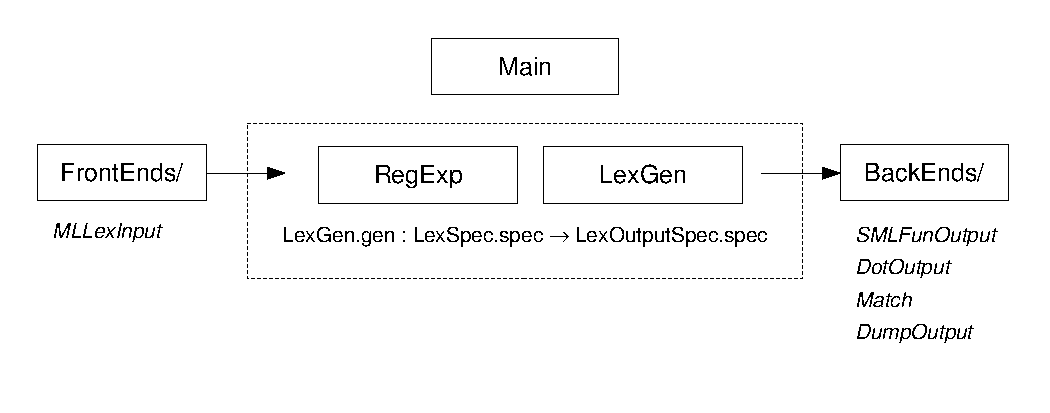
\includegraphics[scale=0.8]{impl-pic.pdf}
\fi
\end{center}
\caption{\ulex{} organization}
\end{figure}

\section{\nm{RegExp}}\label{sec:reg-exp}

In \ulex{}, REs are captured by the abstract type \nm{RegExp.re}.  Introduction
is provided by various ``smart constructors'' (\nm{mkSym}, \nm{mkClosure},
$\dots$), and elimination is provided by the derivatives algorithm.  The
signature for the \rm{RegExp} module is shown below:

\begin{verbatim}
signature REG_EXP =
  sig

    structure Sym : INTERVAL_DOMAIN
    structure SymSet : INTERVAL_SET

    type symbol
    type sym_set
    type re

    val any       : re  (* wildcard *)
    val none      : re  (* EMPTY language *)
    val epsilon   : re  (* the nil character (of length 0) *)

    val mkSym     : symbol -> re
    val mkSymSet  : sym_set -> re

    val mkOr      : re * re -> re
    val mkAnd     : re * re -> re
    val mkXor     : re * re -> re
    val mkNot     : re -> re
    val mkConcat  : re * re -> re
    val mkClosure : re -> re
    val mkOpt     : re -> re
    val mkRep     : re * int * int -> re
    val mkAtLeast : re * int -> re

    val isNone    : re -> bool
    val nullable  : re -> bool
    val derivative : symbol -> re -> re
    val derivatives : re Vector.vector ->
                      ((re Vector.vector) * sym_set) list

    val symToString : symbol -> string
    val toString  : re -> string
    val compare   : re * re -> order

  end
\end{verbatim}

The included structure \nm{SymSet} provides symbol interval sets, which are
ideal when working with dense sets such as unicode character classes.  Interval
set operations (\nm{union}, \nm{complement}, $\dots$) are used extensively;
documentation for the interval set library is available with the SML/NJ
distribution.

Recall that, in using RE derivatives for DFA construction, it is
important to aggresively identify when two REs generate the same
language so that they may be merged to a single state in the automaton.
\nm{RegExp} canonicalizes REs, which is why its \nm{re} type is abstract.
Canonicalization is performed using a lexicographic ordering on REs given by the
\nm{compare} function.  The comparison is lexicographic in the sense that it
first examines the top-level operation of the two REs, and only does more
comparisons if that operation is the same.  We represent REs as follows:
\begin{verbatim}
    datatype re
      = Epsilon
      | Any
      | None
      | SymSet of sym_set
      | Concat of re list
      | Closure of re
      | Op of (rator * re list)
      | Not of re
    and rator = OR | AND | XOR
\end{verbatim}
For the \nm{Op} constructor, which is used for three different commutative
operations, the sub-REs are to be listed in canonical order. The \nm{compare}
function itself will expect that this is the case, and since only smart
constructors can be used to construct REs, the invariant will always hold.

Smart constructors do additional canonicalization beyond ordering.  For
example, \nm{mkNot (mkNot (none))} will be canonicalized
to the same representation as \nm{none}.  Several similar RE equalities
are detected and used.  Also, the smart constructors attempt to push the RE
reprsentation as much toward symbol sets as possible, replacing boolean
operations at the RE level with a single resulting symbol set when possible.
For example, suppose that \nm{AM} held the symbol set for $[A-M]$, \nm{HZ} the
set for $[H-Z]$, and \nm{AZ} the set for $[A-Z]$. Then we would have
\[
\texttt{compare (mkSymSet AZ, mkOr (mkSymSet AM, mkSymSet HZ)) = EQUAL}
\]
The hope is that the cumulative effect of such canonicalization will keep the
generated DFA close to minimal size.

The \nm{derivatve} function constructs a canonicalized derivative for a given
RE with respect to a given symbol; it is a transcription of the algorithm
described in section~\ref{sec:derivatives}.

In general, we will be interested in the derivatives of a vector of REs
(representing the rules in a lexer specification) with respect to \emph{every}
symbol in the alphabet.  As section~\ref{sec:factorings} explains, the unicode
alphabet is too large for us to literally test the derivative at each symbol. 
The \nm{derivatives} function will take a vector of REs and return a list of
\nm{re~Vector.vector~*~sym\_set} \emph{pairs}.  In fact, \nm{derivatives}
is just an implementation of the factor and compress algorithm given
in~\ref{sec:factorings}.  Each pair in the result list represents an arrow
transitioning out of the current state (which corresponds to the input RE
vector) to a new state (the output RE vector) on a given set of symbols (the
output symbol set).  Thus the labor of DFA construction is split between the
\nm{RegExp} module, which computes derivatives (and hence transitions) and
\nm{LexGen}, which actually constructs the DFA graph.

\section{\nm{LexSpec} and \nm{LexOutputSpec}}

Before describing DFA generation, we briefly discuss the relevant input and
output data structures.  The \nm{LexSpec} module has data constructors and
functions relevant to \eg the ML-Lex input specification format, as shown in
Figure~\ref{fig:lex-spec}

\begin{figure}
\begin{verbatim}
    type action = string
    type rule_spec = AtomSet.set option * RegExp.re
    type rule = rule_spec * action

    datatype spec = Spec of {
        decls : string,
        conf : config,
        rules : rule list
      }
\end{verbatim}
\caption{A fragment of \nm{LexSpec}}\label{fig:lex-spec}
\end{figure}

Actions, at least in the present implementation, are just raw strings.  A
\nm{rule} consists of a rule specification and an associated action.  The
optional atom set included with a rule spec represents the start states
to which that rule applies (with \nm{NONE} meaning, strangely enough, all start
states).  With these definitions, a lexer specification is just a list of
rules, some declarations (a raw string containing code) and some miscellaneous
configuration data.

\begin{figure}
\begin{verbatim}
    datatype dfa_state
      = State of {
          id : int,
          label : RegExp.re Vector.vector,
          final : int list,
          next :  (RegExp.sym_set * dfa_state) list ref
        }

    datatype machine = Machine of {
        label : string,
        rules : (RegExp.re * int) vector,
        states : dfa_state list
      }

    type action = string

    datatype spec = Spec of {
        actions : action vector,
        machines : machine list,
        ...  (* configuration data *)
      }
\end{verbatim}
\caption{A fragment of \nm{LexOutputSpec}}\label{fig:lex-output-spec}
\end{figure}

As Figure~\ref{fig:lex-output-spec} illustrates, the output of DFA generation is
\emph{not} a DFA, but a collection of DFAs along with a vector of actions. 
Each \nm{machine} represents a start state for the lexer; that is, each start
state has its own automaton.  However, since start states may use the same
actions, we separate out the actions into a vector so that they are only
emitted once.

A \nm{machine} includes a label, which is just the name of the start state, as
well as the rules relevant to that machine, which are paired with an index to
the associated action in the action vector.  The DFA itself is a list of
states, with the head of the list being $q_0$.  A state, in turn, is labeled by
a vector of REs (with the same length as the \nm{rules} vector in the machine).
 Since a given DFA state may be an accepting state for more than one rule, we
store a \emph{list} of rule indices for the \nm{final} flag.  On a match, the
action for the lowest-index rule is executed first, but that action may use
\nm{REJECT()}, in which case it may be necessary to jump to the action for the
next rule index given in the \nm{final} list.

\section{\nm{LexGen}}\label{sec:lex-gen}

\nm{LexGen} is a very simple module with a single accessible function:
\begin{center}
\nm{gen : LexSpec.spec -> LexOutputSpec.spec}
\end{center}

The first task of the \nm{gen} function is to collate the actions and start
states.  The actions from the input spec are separated from their rules into a
vector.  Afterwards, \nm{gen} iterates over the specified start states,
collecting the rules for each start state and using the \nm{mkDFA} function to
generate a machine for each.

\nm{mkDFA} performs a straightforward imperative DFA construction, using
the \nm{derivatives} function from \nm{RegExp} to compute the transitions out of
each node. A map of RE vectors to DFA nodes is maintained (using
\nm{Vector.collate RegExp.compare} for ordering); this map is used to recognize
when a new out-edge is going to an existing DFA node.  Finally, any transition
to a vector of REs which all generate the empty language is an error transition
(that is, the derivatives for the given transition symbol set all indicate a
non-match).

\section{Front ends}

At the moment, only one front end is available: the ML-Lex specification
format.  Eventually \ulex{} will have its own format.

The ML-Lex front end is fairly straightforward: it uses ML-Yacc to do the
parsing, and can use either ML-Lex or \ulex{} to do the lexing.  The
distribution includes a lexer that was generated from \ulex{} to serve as a
bootstrap.

\section{Back ends}

One exciting aspect of \ulex{} is the ability to easily add back ends.  The
following back ends are currently included in the distribution.

\paragraph{SML control-flow lexer generation}

The most important back end is code generation for SML.  At present, there is a
single code generation strategy: build a lexer using control-flow (\ie
if statements and tail-calls) to match the input.  If the control-flow strategy
turns out to be inadequate, it would be fairly easy to add a code
generator for table-based lexing.

Code generation is performed by expanding stubs in a template SML file.  The
template contains code for dealing with streams and setting up the lexer in the
appropriate way.  Input is read from functional strings, which allow for
the arbitrary lookahead needed for maximal-munch.  These streams also track
the current file position and line number.

A helper module, \nm{ML}, contains a representation for a good portion of the
Standard ML expression langauge, and support for pretty-printing such
expressions.

The generated code includes user actions and the DFA for each start state.
 Within each start state there is one \emph{state function} per DFA node.  Each
state function will examine the next character of input and perform a series of
if-tests to determine the correct transition.  The if-tests perform a
hard-coded binary search over the symbol set intervals for the transitions.

The lexer stores a reference cell for the current functional stream.  Each time
the lexer accepts a token, the cell is updated.  \nm{yytext} is generated (only
when needed) by ``subtracting'' the new stream from the one stored in the
reference cell before updating it.  Subtraction simply rescans the appropriate
number of characters from the stored stream, which should still have the string
in its buffer.

One subtlety is handling calls to \nm{REJECT()}.  Since such calls are fairly
rare, we want to avoid tracking the information \nm{REJECT} needs if it won't
be used.  \nm{REJECT} information consists of (in essence) a list of all the
previous matches.  A previous match could occur on the same DFA state if
multiple REs matched the input at that state; otherwise, the previous match is
a prefix of the \nm{REJECT}ed match.  Whenever a transition is made, the
appropriate previous match information is passed up to the next state. 
However, if the current state is an accepting state that does not use
\nm{REJECT}, then the history is \emph{truncated} at the \nm{REJECT}-free
point, since it could never be used.  This determination is made statically and
is hard-coded into the generated SML lexer.

\paragraph{Graphviz}

The Graphviz toolkit provides easy graph visualization using a very simple
graph description format.  We utilize the DOT format.  The Graphviz backend
will write one DOT file for each start state, showing all nodes for that start
state's DFA, along with labeled transitions.  See \texttt{www.graphviz.org} for
details on the DOT format.

\paragraph{Text dump}

If Graphviz is not available or a more detailed summary is desired, the
\nm{DumpOutput} module can be used to print to standard out every DFA state,
labeled by its RE vector, along with out-edges, for every start state in the
lexer.

\paragraph{Interactive matching}

Finally, a simple interactive back end is available.  Interactive matching
allows a user to enter arbitrary strings and find out (1) if they matched and
(2) what RE matched them.  The code for interactive matching is quite simple.

\section{\nm{Main}}

The \nm{Main} module is the driver for \ulex{}: it is responsible for processing
command-line arguments and hooking up the appropriate front and back ends. 
Since it is very simple, it gives a nice overview of the system and is a good
place to look first in trying to undertand the code.
		\chapter[\mlantlr]{Code: \mlantlr}

\backmatter

	\bibliographystyle{plain}
	\bibliography{deriv.bib}

\end{document}
